\section{Motivating example}\label{sec:example}

%%%%%%%%%%%%%%%%%%%%%%%%%%%%%%%%%%%%%%%%%%%%%%%%%%%%%%%%%%%%%%%%%%%%%%
%% BACKGROUND ON KAPPA
%%%%%%%%%%%%%%%%%%%%%%%%%%%%%%%%%%%%%%%%%%%%%%%%%%%%%%%%%%%%%%%%%%%%%%

\subsection{Some background on Kappa}

Stochastic simulations of Kappa models can be run using the Gillespie
algorithm, which is summarized Listing~\ref{alg:gillespie}.

\begin{algorithm}
\caption{Doob-Gillespie algorithm}\label{alg:gillespie}
\begin{spacing}{1.2}
\begin{algorithmic}
\vspace{0.2cm}
  \STATE $t \gets 0$
  \STATE $m \gets\ $ initial mixture
  \vspace{0.1cm}
  \WHILE{ $t < t_\text{\,end}$ }
      \vspace{0.1cm}
      \STATE $\alpha \gets \sum_r {\lambda_r |\EMBS{r}{m}|}$
      \vspace{0.1cm}
      \STATE draw $\delta \sim \textsc{Exp}(\alpha) $
      \STATE $t \gets t + \delta$
      \STATE draw a rule $r$ with probability
      $\propto \ \lambda_r |\EMBS{r}{m}|$
      \STATE draw an embedding $\xi$ uniformly in $\EMBS{r}{m}$
      %\STATE update $m$ by triggering event $((r, \xi), t)$
      \STATE $m \gets \UPDATE{m}{(r, \xi)}$
      \STATE log event $((r, \xi), t)$
  \ENDWHILE
\vspace{0.1cm}
\end{algorithmic}
\end{spacing}
\end{algorithm}

In Gillespie's algorithm, the activity of a rule $r$ is defined as the
product $\lambda_r|\EMBS{r}{M}|$ of its reaction rate by the number of
embeddings of its left hand side in the current reaction mixture.
Then, simulating a trace works by repeating the following steps:
\begin{inparaenum}[1)]

\item draw the time before the next simulation event from an
  exponential distribution of parameter the total activity $\alpha$ of
  the rules and increment the current time by this amount
\item draw a rule $r$ with probability proportional to its activity
\item pick an instance of the left hand side of $r$ uniformly in the
  current mixture and rewrite it.
\end{inparaenum}


%%%%%%%%%%%%%%%%%%%%%%%%%%%%%%%%%%%%%%%%%%%%%%%%%%%%%%%%%%%%%%%%%%%%%%
%% TRADITIONAL PATHWAY ANALYSIS FALLS SHORT
%%%%%%%%%%%%%%%%%%%%%%%%%%%%%%%%%%%%%%%%%%%%%%%%%%%%%%%%%%%%%%%%%%%%%%

\subsection{Where traditional pathway analysis falls short}

% Much more to say about Kappa

We illustrate the need for counterfactual reasoning on a toy example
in Kappa. Consider a model with two types of agents, kinases $K$ and
substrates $S$, interacting according to the rules depicted in
Figure~\ref{fig:model}.

% -*- TeX-master: "ijcai18.tex" -*-

\begin{figure}[h]
  \vskip -0.2cm
  \begin{center}
    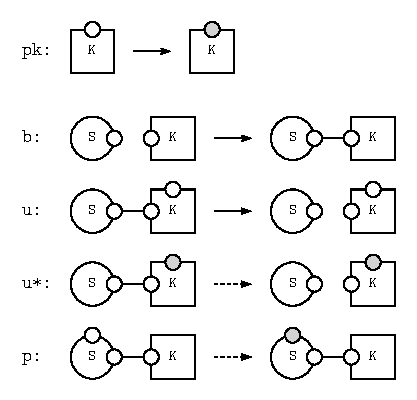
\includegraphics[scale=0.9]{figures/model.pdf}
  \end{center}
  \vskip -0.2cm
  % \caption{A motivating toy model. As usual in Kappa, sites not
  %   mentioned in a rule are left unchanged by it. Instead of naming
  %   sites, we here identify them by their position on an
  %   agent. Phosphorylated sites are shown in gray. Firing rates are
  %   not specified here but dotted arrows indicate \textit{slow}
  %   reactions, whereas solid arrows indicate \textit{fast} reactions.}
  \caption{A motivating toy model. Sites not mentioned in a rule are
    left unchanged by it. \longversion{As in
      Figure~\protect\ref{fig:mixture}, sites are identified by their
      position on an agent.}  Firing rates are not specified, but
    dotted (solid) arrows indicate \textit{slow} (\textit{fast})
    reactions
    $(\lambda_u \gg \lambda_{u^*} \approx \lambda_p)$.}
  \label{fig:model}
\end{figure}


For the sake of simplicity, consider an initial mixture $I$ with only
a single kinase and a single substrate whose sites are free and
unphosphorylated. We then ask: Starting from $I$, \textbf{how} is $p$
triggered ? We are not merely looking for an account of reachability
but rather for causal narratives, that is, collections of necessary
events connected by causal influences.

A stochastic simulation \cite{DanosEtAl-APLAS07} might produce the
following trace (events are labelled by the rules that induced them):
\begin{align}\label{example-trace} b,\ \ u,\ \ pk,\ \ b,\ \ p,\ \
  u^{*},\ \ \cdots
\end{align} Figure~\ref{fig:dumb-story} depicts the causal narrative
explaining the occurrence of $p$ according to existing techniques
\cite{DBLP:conf/fsttcs/DanosFFHH12,DanosEtAl-CONCUR07}. The arrow
between $b$ and $p$ is called an \textit{activation arrow}, meaning
that $b$ modifies an aspect of state (by creating a link) that enables
$p$ to happen.

\begin{figure}[H]
  \vskip -0.8cm
  \begin{center}
    \includegraphics[scale=0.7]{figures/dot/dumb-story.pdf}
  \end{center}
  \vskip -1cm
  \caption{A causal explanation for $p$ in trace
    (\ref{example-trace}).  Events are labelled by the rules that
    induced them. The \emph{init} node corresponds to a special event
    that sets the mixture to its initial state.  }
  \label{fig:dumb-story}
\end{figure}


This narrative, however, is blind to the critical role of $pk$ in the
original trace. Looking at the rules in Figure~\ref{fig:model} one
notes that:
\begin{inparaenum}[(i)]
\item the phosphorylation rule $p$ is slow
\item the average time $K$ and $S$ remain bound depends on whether $K$
  is phosphorylated, as manifest in the two unbinding rules $u$ (fast,
  if $K$ is not phosphorylated) and $u^{*}$ (slow, if $K$ is
  phosphorylated).
\end{inparaenum} It seems reasonable to assert that $p$ would probably
not have happened had $pk$ not happened, as the opportunity for $p$
would have been cut short by a fast unbinding event. We therefore
argue that $pk$, although it does not activate $b$ or $p$ directly,
should be part of a causal narrative for $p$. Reasoning of this kind
is \textit{counterfactual} and can be deployed to define causality
\cite{lewis1974causation,lewis2000causation}.

In section~\ref{sec:counterfactual}, we give a rigorous semantics to
this line of reasoning. In section~\ref{sec:inhibition} we show that
counterfactual statements can be expressed using inhibition arrows,
leading to the explanation shown in Figure~\ref{fig:cex}.

% Therefore, although the causal relevance of $pk$ cannot be justified
by activation arrows, it is supported by a counterfactual statement.
% In the rest of this abstract, we %give a formal semantics to
counterfactual statements and investigate how %they can be used %to
produce more satisfying causal explanations.